\section{Aprendizado de Máquina e Algoritmos}\label{sec:LABEL_CHP_4_SEC_A}


Conhecido também pelo termo em inglês Machine Learning, é a capacidade da máquina através de um algoritmo computacional, desempenhar funções cognitivas geralmente associadas a mente humana, tais como aprender, identificar padrões e resolver problemas complexos\cite{michalski2013machine}. O aprendizado de máquina tem como principal objetivo extrair informações de dados fornecidos, e então desenvolver um modelo genérico suficiente, que é capaz de responder de maneira apropriada um problema proposto.

O aprendizado de máquina pode ser agrupado em três categorias: Aprendizado Supervisionado, Não Supervisionado e Reforçado. Além disso, esses grupos podem ser subclassificados como Aprendizado Passivo ou Aprendizado Ativo. Um algoritmo pode ser do tipo Supervisionado Passivo ou Supervisionado e Ativo, por exemplo.

Algumas das principais etapas do aprendizado de máquina estão no fluxograma da Figura \ref{fig:tipos-aprendizado},  além disso essas atividades são usadas em diferentes tipos de aprendizado, que serão discutidos a seguir.


\begin{figure}[ht]
    \centering
    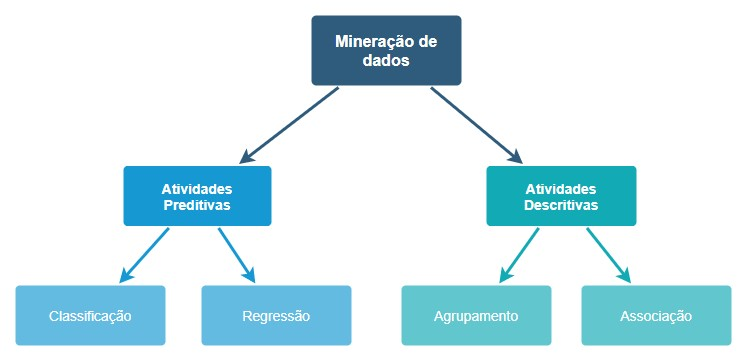
\includegraphics[height=7.5cm]{tipos-aprendizado.jpg} 
    \caption{Atividades de aprendizado de máquina}
    \label{fig:tipos-aprendizado}
\end{figure}

\pagebreak

\subsection{Aprendizado supervisionado}\label{sec:LABEL_CHP_4_SEC_A_SUB_A}

No aprendizado supervisionado supõe-se que os objetos de uma categoria ou classe compartilham características comuns, semelhantes, que proporcionam informações suficientes para o algoritmo conseguir distinguir e classificar uma nova informação não observada antes. Um especialista é responsável por preparar os parâmetros de entrada do algoritmo e observar o resultado de saída, e avaliar se a resposta obtida pelo modelo condiz com o esperado, e caso necessário o especialista ajusta novamente os parâmetros do modelo, a Figura \ref{fig:aprendisado-supervisionado} ilustra esse conceito.



\begin{figure}[ht]
    \centering
    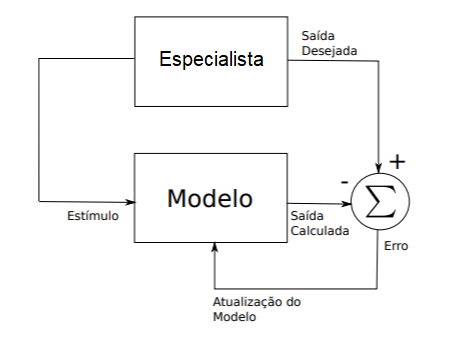
\includegraphics[height=5.2cm]{aprendizado-supervisionado.png} 
    \caption{ Aprendizado Supervisionado. Adaptado de \cite{de2007redes}}
    \label{fig:aprendisado-supervisionado}
\end{figure}

Neste aprendizado temos basicamente a regressão e a classificação \cite{dangeti2017statistics}. Na regressão o valor a ser previsto é uma variável numérica contínua, como por exemplo, o preço de um imóvel, temperatura prevista para uma data. E na classificação, será previsto uma categoria, como por exemplo se um e-mail é spam ou não, se um caractere em uma imagem é uma letra ou numero, ou para o caso deste trabalho qual a fase esperada para uma determinada composição de uma liga.

\subsection{Aprendizado não supervisionado}\label{sec:LABEL_CHP_4_SEC_A_SUB_B}

No aprendizado não supervisionado os dados são utilizados para estímulo do algoritmo, isto é, para treinamento do modelo, podem ou não estar acompanhados dos dados desejados para a saída. Além disso, nesse caso não há a figura do ``especialista'' e não é feito nenhum procedimento de correção do erro (Figura \ref{fig:aprendizado-nao-supervisionado}). O modelo observa os padrões e correlações das informações disponibilizadas e agrupa o conjunto de dados em classes.

\begin{figure}[ht]
    \centering
    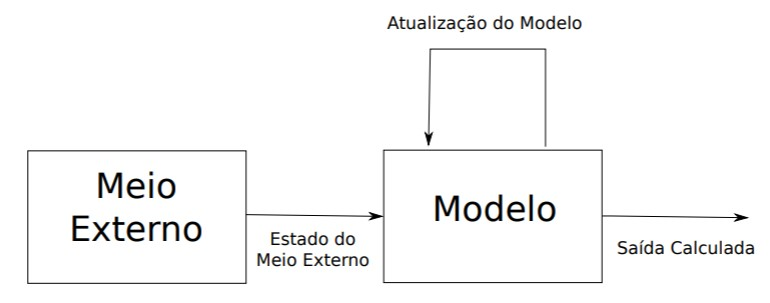
\includegraphics[height=4.2cm]{aprendizado-nao-supervisionado.jpg} 
    \caption{ Aprendizado não supervisionado. Adaptado de \cite{de2007redes}}
    \label{fig:aprendizado-nao-supervisionado}
\end{figure}
\FloatBarrier

\subsection{Aprendizado por reforço}\label{sec:LABEL_CHP_4_SEC_A_SUB_C}

O aprendizado por reforço é um mecanismo onde o modelo segue um ciclo baseado em observação, ação, recompensa e novo estado, pode ser descrito como um processo de Markov \cite{fernando2020cadeiaMarkov}, este processo possui as seguintes informações:

\begin{itemize}
    \item E:  espaço de estados
    \item A:  espaço de ações
    \item R:  função de recompensas \\
    $R(e,a): E \times A \rightarrow \mathbb{R}$
    \item T:  função de transição de estado \\ 
    $T(e,a,e'): E^2 \times A \rightarrow [0,1]$ \\
    $T(e,a,e') = p(e'|e,a)$
    \item $\gamma$: fator de ajuste entre recompensas de curto e longo prazo
\end{itemize}


O principal objetivo é maximizar a recompensa obtida a partir de uma função de escolha $\pi(e): E \rightarrow A$

\begin{figure}[ht]
    \centering
    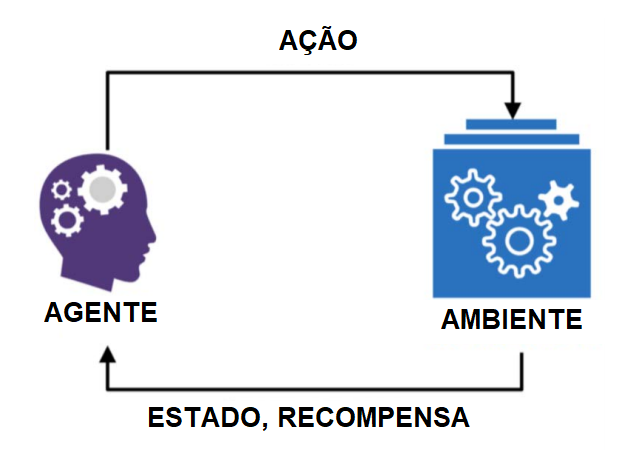
\includegraphics[height=6cm]{aprendizado-reforcado.png} 
    \caption{ Aprendizado reforçado.}
    \label{fig:aprendizado-reforcado}
\end{figure}
\FloatBarrier


\subsection{Classificação}\label{sec:LABEL_CHP_4_SEC_A_SUB_D}


Um problema é linearmente separável se existe um hiperplano capaz de separar completamente as classes. Quanto maior a separabilidade das classes, menor a complexidade do problema \cite{smola2008introduction}, na Figura \ref{fig:complexidade-sistema} pode-se observar os tipos de complexidade de dados.

\begin{figure}[ht]
    \centering
    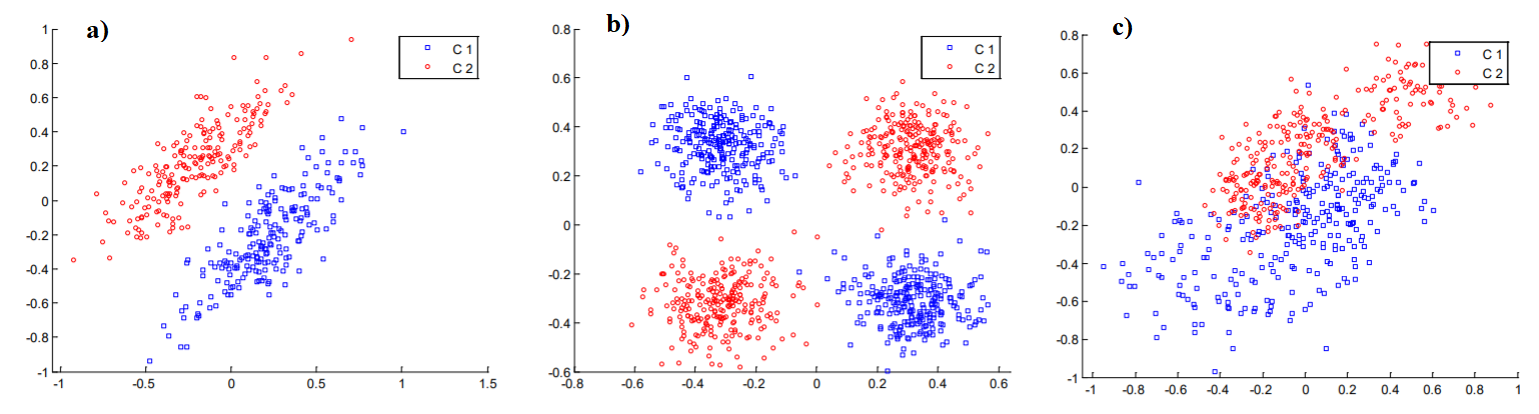
\includegraphics[height=4.2cm]{complexidade-sistema.png} 
    \caption{ a) Linearmente separável b) Separável não linearmente c) Não separável}
    \label{fig:complexidade-sistema}
\end{figure}
\FloatBarrier

Um algoritmo classificador possui a capacidade de rotular uma nova informação proposta ao modelo baseando-se no padrão dos dados de um conjunto previamente observado. Além disso para mensurar a qualidade do algoritmo classificador são realizadas algumas avaliações como a performance, precisão, acurácia e outras métricas de avaliação do mesmo.




\subsection{Regressão}\label{sec:LABEL_CHP_4_SEC_A_SUB_E}

 O objetivo da regressão é o desenvolvimento de um modelo capaz de identificar o valor mais correto possível para um novo conjunto de entradas.



\begin{figure}[ht]
    \centering
    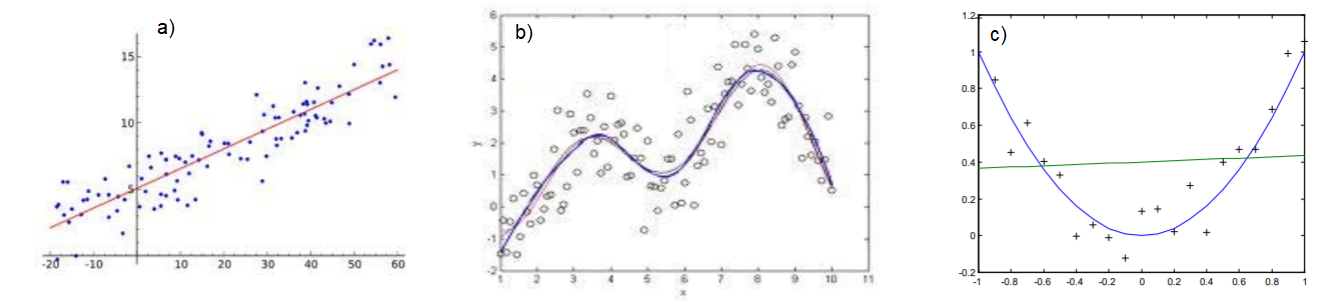
\includegraphics[width=16cm]{regressoes.png} 
    \caption{ a) Linear b) Não Linear c) Polinomial}
    \label{fig:regressoes}
\end{figure}
\FloatBarrier

\pagebreak
\subsection{Ajuste de modelo}\label{sec:LABEL_CHP_4_SEC_A_SUB_F}

Quando algoritmos de aprendizado de máquina são construídos, o conjunto de dados de uma amostra é utilizado para treinar o modelo. No entanto, dependendo de da forma que o modelo foi ajustado aos dados, como por exemplo, o tempo de treinamento, a complexidade do modelo, falta ou excesso de variáveis, poderá ocorrer consequências nos resultados se não houver um equilíbrio no ajuste do modelo, isto é, um cenário de underfitting ou overfitting.

\begin{figure}[ht]
    \centering
    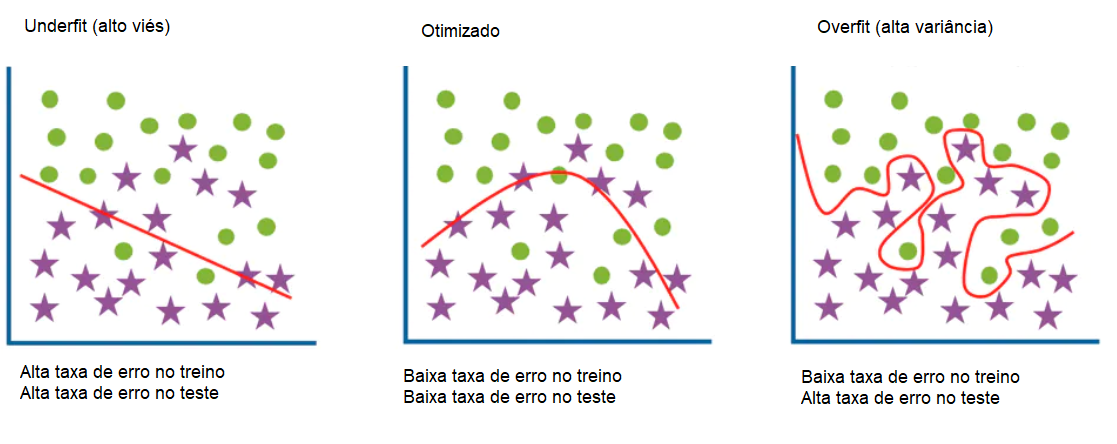
\includegraphics[height=6cm]{overfitting-underfitting.png} 
    \caption{Overfitting vs. underfitting. Adaptado de \cite{art:overfitting} }
    \label{fig:fitting-underfitting}
\end{figure}
\FloatBarrier

Em ambos os cenários, o modelo não é capaz de estabelecer a tendência dominante no conjunto de dados de treinamento. Como resultado, o underfitting também generaliza mal para dados não vistos. No entanto, ao contrário do overfitting, os modelos subajustados apresentam alta polarização e menos variação em suas previsões. Isso demonstra a relação inversamente proporcional de viés-variância, que ocorre quando um modelo subajustado muda para um estado superajustado. À medida que o modelo aprende, seu viés reduz, mas pode aumentar a variância à medida que se torna excessivamente ajustado. Ao ajustar o modelo, o objetivo é encontrar o ``ponto ideal'' entre sub e sobre ajuste, para que possa estabelecer uma tendência dominante e aplicá-la amplamente a novos conjuntos de dados.

\subsubsection{Overfitting}\label{sec:LABEL_CHP_4_SEC_A_SUB_F_A}
Overfitting é um conceito em ciência de dados, onde, um modelo é ajustado excessivamente e começa a aprender o ``ruído'', ou informação irrelevante, dentro do conjunto de dados. Quando isso acontece, o algoritmo se torna incapaz de classificar ou prever dados nunca antes vistos, isso significa uma baixa generalização do modelo. 

Baixas taxas de erro e alta variância são bons indicadores de overfitting. Para evitar esse tipo de comportamento, parte do conjunto de dados de treinamento é separada como um ``conjunto de teste'' para verificar a ocorrência de overfitting. Quando os dados de treinamento apresentarem baixa taxa de erro, e os conjunto de teste tiverem uma alta taxa de erro, é um claro sinal de overfitting.

\subsubsection{Underfitting}\label{sec:LABEL_CHP_4_SEC_A_SUB_F_B}
Por outro lado, quando é observado underfitting, o modelo não é capaz de capturar a relação entre as variáveis de entrada e saída com precisão, resultando numa alta taxa de erros em tanto para o conjunto de treinamento quanto para dados não vistos. Isso ocorre quando um modelo é muito simples, é resultado de um modelo que precisa de mais tempo de treinamento, mais recursos de entrada, ou menos regularização. Assim como o overfitting, é o mal ajuste de um modelo, onde ele não é capaz de estabelecer uma tendência na maioria dos dados, e consequentemente, resultando em erros no treinamento e baixo desempenho no modelo ao classificar ou prever dados novos.


\subsection{Validação cruzada}\label{sec:LABEL_CHP_4_SEC_A_SUB_G}

Avaliar um conjunto de dados de tamanho limitado é uma tarefa muito desafiadora. Ao separar o conjunto de dados em treino e teste, podemos ter overfitting no conjunto de testes porque os parâmetros podem ser ajustados até que o estimador tenha um desempenho ideal. Isto significa que o conjunto de teste deixa de representar uma amostra generalizada. Para contornar essa situação, podemos separar uma outra parte do conjunto de dados para ser o ``conjunto de validação'': o treinamento continua no conjunto de treinamento, logo após é utilizado o conjunto de validação para verificar se o ajuste do modelo foi bem sucedido, e por fim é feita a avaliação do modelo com o conjunto de teste.

No entanto, ao particionar o conjunto de dados em três conjuntos, reduzimos drasticamente o número de amostras disponíveis para o treinamento do modelo, isto é uma penalidade ainda maior quando consideramos um conjunto de dados bastante limitado.

\pagebreak

Uma solução para esse problema é o uso da validação cruzada (também conhecida como cross validation em inglês). Neste caso um conjunto de teste ainda é utilizado na avaliação final, porém não é necessário o uso de um conjunto de validação. O conjunto de treinamento é dividido em $k$ conjunto menores, então o modelo é treinado com $k-1$ das divisões do conjunto, porém em $k$ etapa do treinamento o conjunto de teste é diferente\cite{art:cross-validation}.


\begin{figure}[ht]
    \centering
    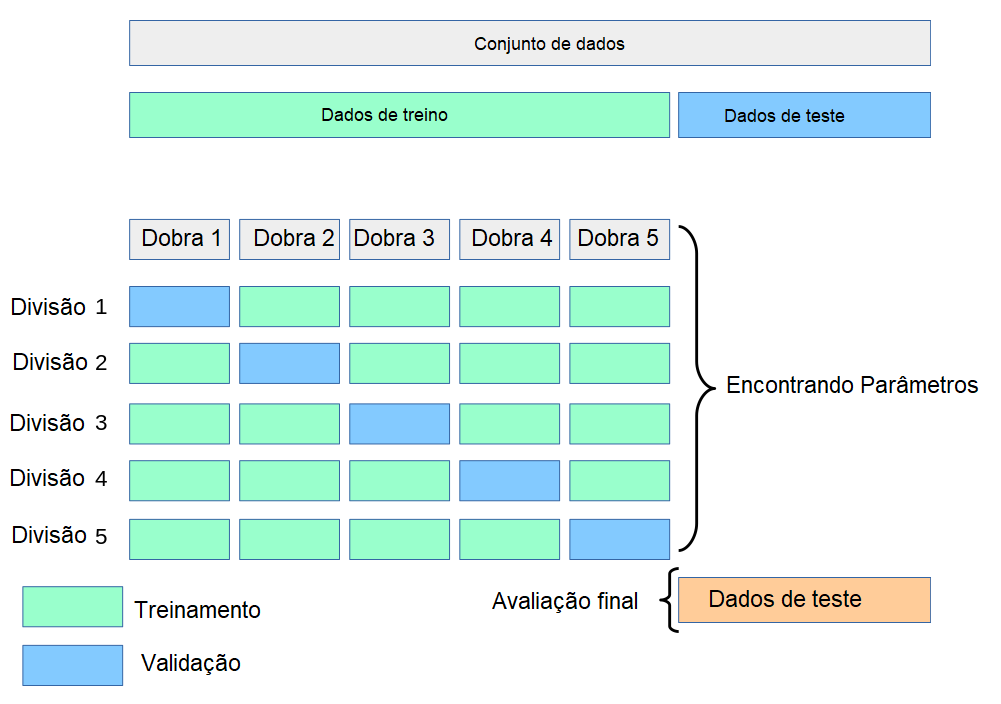
\includegraphics[height=8cm]{grid_search_cross_validation.png} 
    \caption{Ciclos do algoritmo de validação cruzada}
    \label{fig:crossv}
\end{figure}
\FloatBarrier



\subsection{Métricas de avaliação}\label{sec:LABEL_CHP_4_SEC_A_SUB_H}

Após criarmos um modelo de classificação, é necessário verificar a qualidade do modelo, para isso, são utilizadas algumas métricas, que por sua vez, usam a relação entre a previsão do modelo e os dados reais dando origem a uma matriz de confusão (Figura \ref{fig:matriz_confusao}).

\begin{figure}[ht]
    \centering
    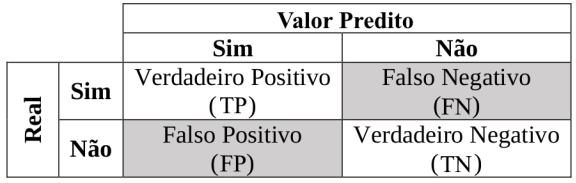
\includegraphics[height=4cm]{matriz_confusao.png} 
    \caption{Matriz de confusão}
    \label{fig:matriz_confusao}
\end{figure}
\FloatBarrier

\begin{itemize}
    \item Positivo Verdadeiro (True Positive – TP) que significa que a classe prevista e observada originalmente fazem parte da classe positiva;
    \item Falso Positivo (False Positive – FP) que significa que a classe predita retornou positivo mas a original observada era negativa;
    \item Negativo Verdadeiro (True Negative – TN) os valores preditos e observados fazem parte da categoria negativa;
    \item Falso Negativo (False Negative – FN) representa que o valor predito resultou na classe negativa mas o original observado era da classe positivo.
\end{itemize}

Com base nos resultados da matriz de confusão os valores das métricas podem ser calculados.

\begin{itemize}
    \item Acurácia (Acurary): Quantidade classificada como Positivos e Negativos corretamente, e pode ser formalizada em (TP + TN) / (TP + TN + FP + TN)
    \item Precisão (Precision): Quantidade Positiva classificada corretamente. E é calculada por TP / (TP + FP)
    \item Recall: Taxa de valores classificada como Positivo, comparada com quantos deveriam ser. E pode ser calculada como  \\
    $TP / (TP + FN)$
    \item F1 SCORE: É calculado como a média harmônica entre Precisão e Recall, sendo sua formulação matemática representada por \\ 
    (2* TP) / (2* TP + FP + FN) 
\end{itemize}


\subsection{Correlação }\label{sec:LABEL_CHP_4_SEC_A_SUB_H}

O coeficiente de correlação $\tau$ de Kendall é uma das medidas utilizadas mais comuns para calcular a quantidade de correlação entre duas classificações. Sejam $( x_j, y_j )$ e $( x _ { k } , y _ { k } )$ dois elementos de uma amostra $\{ ( x _ { i } , y _ { i } ) \} _ { i = 1 } ^ { n }$ de uma população bivariada, ou seja, quando duas variáveis de uma população apresentam um comportamento na presença uma da outra. Temos  $( x_j, y_j )$ e $( x _ { k } , y _ { k } )$ são concordantes se $x _ { j } < x _ { k }$ e $y _ { j } < y _ { k }$ ou se $x _ { j } > x _ { k }$ e $y _ { j } > y _ { k }$ (ou seja, se $( x _ { j } - x _ { k } ) ( y _ { j } - y _ { k } ) > 0$); e discordante se $x _ { j } < x _ { k }$ e $y _ { j } > y _ { k }$ e se $x _ { j } > x _ { k }$ e $y _ { j } < y _ { k }$ (ou seja, se $( x _ { j } - x _ { k } ) ( y _ { j } - y _ { k } ) < 0$). 

Existem $\left( \begin{array} { l } { n } \\ { 2 } \end{array} \right)$ pares distintos de observações na amostra, e cada par (exceto empates) é concordante ou discordante. Denotado por $S$ o número $c$ de pares concordantes menos o número $d$ pares discordantes, o $\tau$ de Kendall para amostra é definido como na Equação \ref{eq:tau-kendall} \ref{eq:tau-kendall} \cite{art:kendall2010}\cite{kendall1938new} \cite{kendall1970rank}.

\begin{equation} 
\tau _ { n } = \frac { c - d } { c + d } = \frac { S } { \left( \begin{array} { l } { n } \\ { 2 } \end{array} \right) } = \frac { 2 S } { n ( n - 1 ) }
\label{eq:tau-kendall}
\end{equation}

Quando empates existem nos dados, é utilizado o seguinte ajuste conforme a Equação \ref{eq:tau-kendall-empate}.

\begin{equation} 
\tau _ { n } = \frac { S } { \sqrt { n ( n - 1 ) / 2 - T } \sqrt { n ( n - 1 ) / 2 - U } }, \label{eq:tau-kendall-empate}
\end{equation}

Onde $T = \sum _ { t } t ( t - 1 ) / 2$  para $t$ o número de $X$ observações que são empatadas em uma dada classificação, e $U = \sum _ { u } u ( u - 1 ) / 2$ para $u$ o número de $Y$ observações que são empatadas em uma dada classificação. 



